\section{Environment 1A}

\lipsum[1-4]
%\lipsum[1-5] this breaks it, fills first column

\begin{chart}{S}{ll}
\caption{Incarceration ratest across countries}
\label{chart:incarceration}
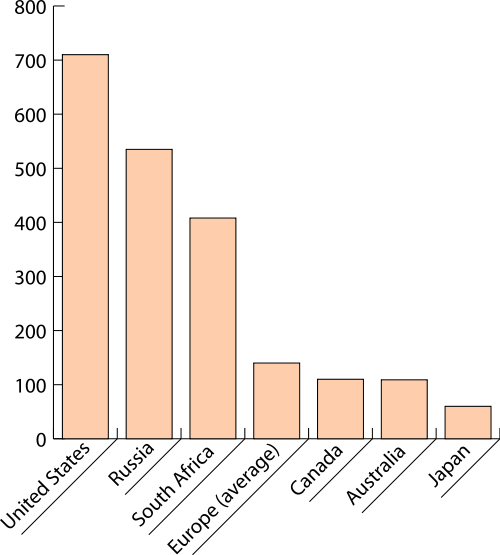
\includegraphics[width=\chartwidth,height=\chartheight]{incarceration}  
\source{Wikipedia}
\end{chart}

\begin{chart}{S}{lr}
\caption{Incarceration ratest across countries}
\label{chart:incarceration}
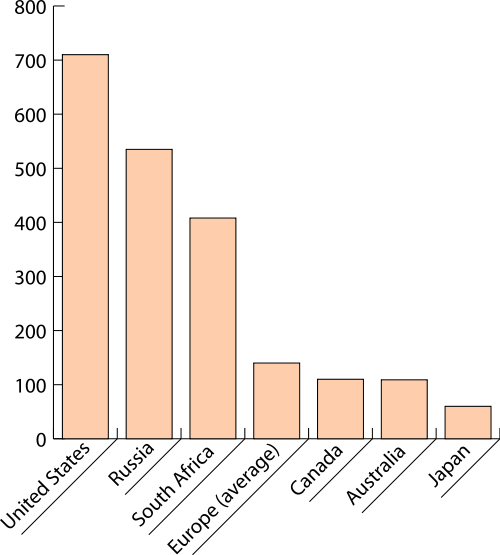
\includegraphics[width=\chartwidth,height=\chartheight]{incarceration}  
\source{Wikipedia}
\end{chart}

\begin{map}{W}{UL}
\caption{Ancient Roma  (Trajan times)}
\label{map:roma}
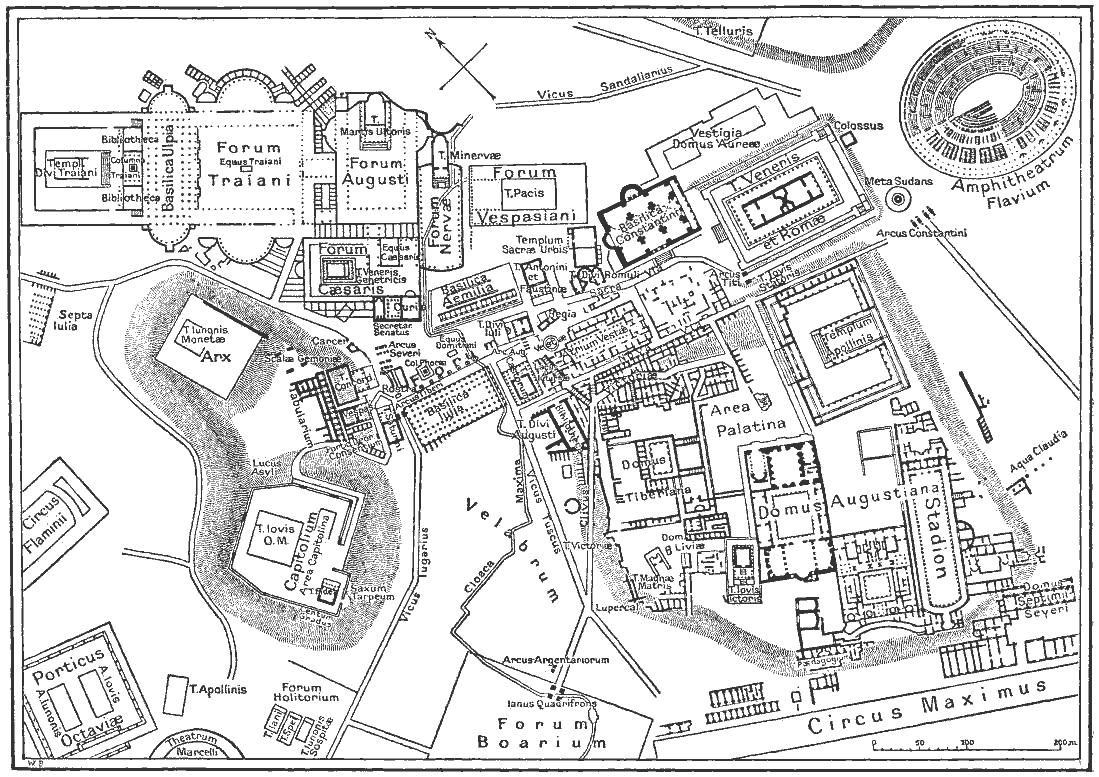
\includegraphics[width=\chartwidth,height=\chartheight]{Rome}
\source{Wikipedia}
\refMetadata{agripop}
\end{map}

\begin{chart}{S}{LL}
\caption{Incarceration ratest across countries}
\label{chart:incarceration}
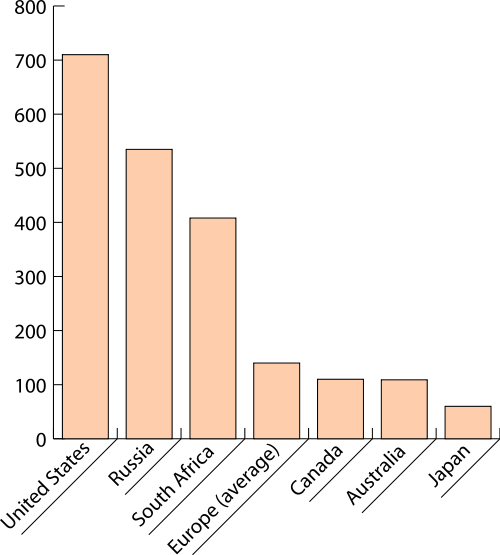
\includegraphics[width=\chartwidth,height=\chartheight]{incarceration}  
\source{Wikipedia}
\end{chart}

\begin{chart}{S}{LR}
\caption{Incarceration ratest across countries}
\label{chart:incarceration}
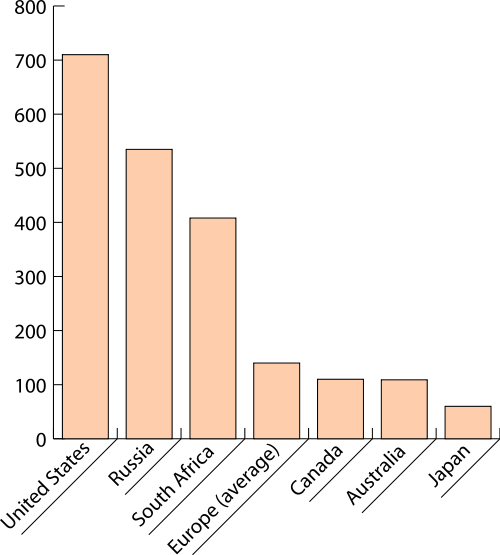
\includegraphics[width=\chartwidth,height=\chartheight]{incarceration}  
\source{Wikipedia}
\end{chart}

%\section{Environment 1B}
%
%\lipsum[1-4]
%%\lipsum[1-5] this breaks it, fills first column
%
%\begin{chart}{S}{ll}
%\caption{Incarceration ratest across countries}
%\label{chart:incarceration}
%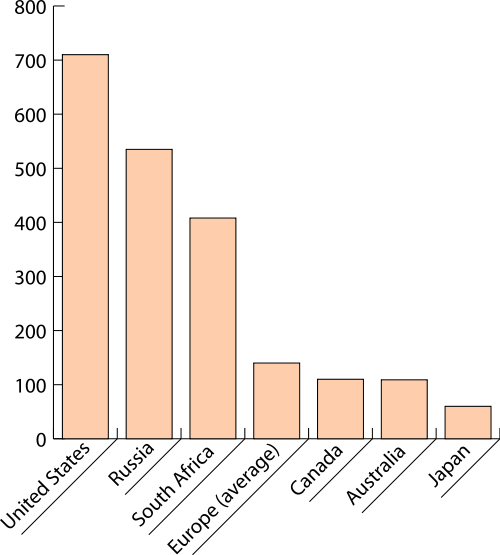
\includegraphics[width=\chartwidth,height=\chartheight]{incarceration}  
%\source{Wikipedia}
%\end{chart}
%
%\begin{chart}{S}{lr}
%\caption{Incarceration ratest across countries}
%\label{chart:incarceration}
%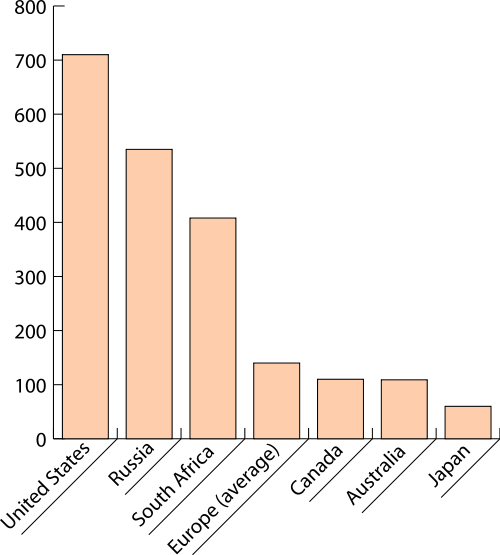
\includegraphics[width=\chartwidth,height=\chartheight]{incarceration}  
%\source{Wikipedia}
%\end{chart}
%
%\begin{chart}{S}{UL}
%\caption{Incarceration ratest across countries}
%\label{chart:incarceration}
%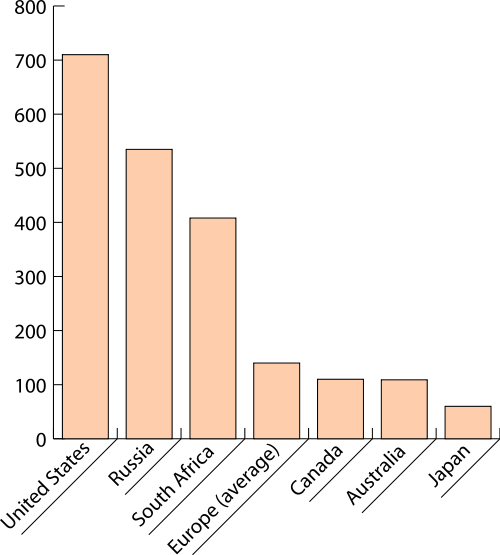
\includegraphics[width=\chartwidth,height=\chartheight]{incarceration}  
%\source{Wikipedia}
%\end{chart}
%
%\begin{chart}{S}{UR}
%\caption{Incarceration ratest across countries}
%\label{chart:incarceration}
%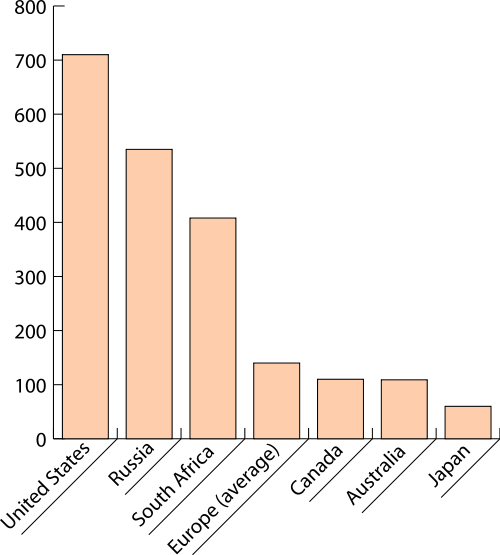
\includegraphics[width=\chartwidth,height=\chartheight]{incarceration}  
%\source{Wikipedia}
%\end{chart}
%
%\begin{map}{W}{LL}
%\caption{Ancient Roma  (Trajan times)}
%\label{map:roma}
%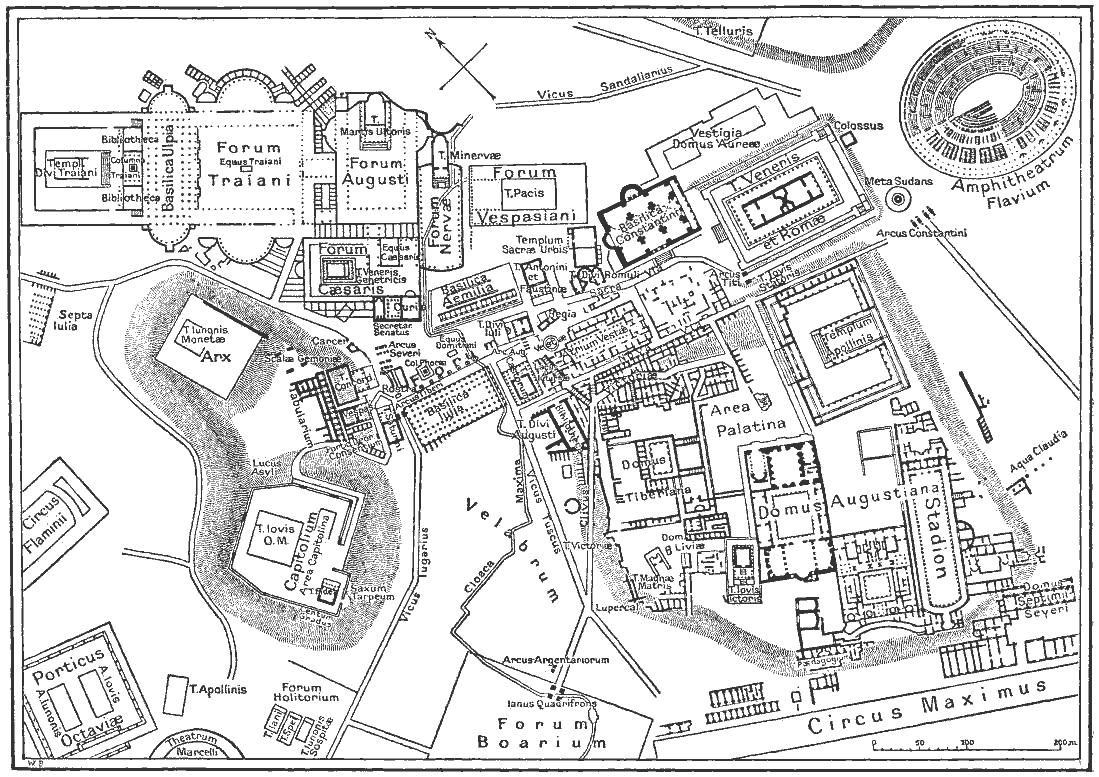
\includegraphics[width=\chartwidth,height=\chartheight]{Rome}
%\source{Wikipedia}
%\refMetadata{agripop}
%\end{map}


%%%%%%%%%%%%%%%%%%%%

\section{Environment 1C}

\lipsum[1-4]
%\lipsum[1-5] this breaks it, fills first column

\begin{chart}{S}{ll}
\caption{Incarceration ratest across countries}
\label{chart:incarceration}
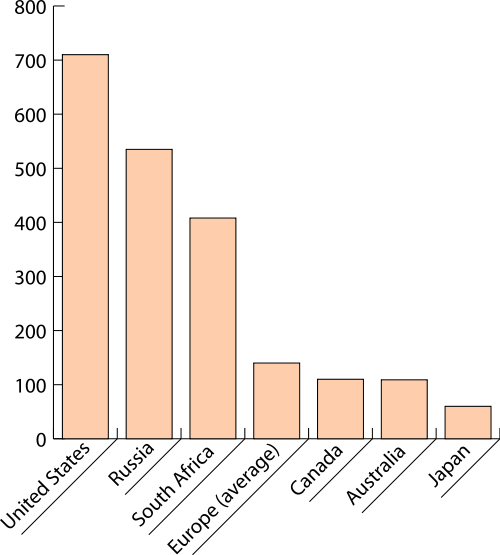
\includegraphics[width=\chartwidth,height=\chartheight]{incarceration}  
\source{Wikipedia}
\end{chart}

\begin{chart}{S}{lr}
\caption{Incarceration ratest across countries}
\label{chart:incarceration}
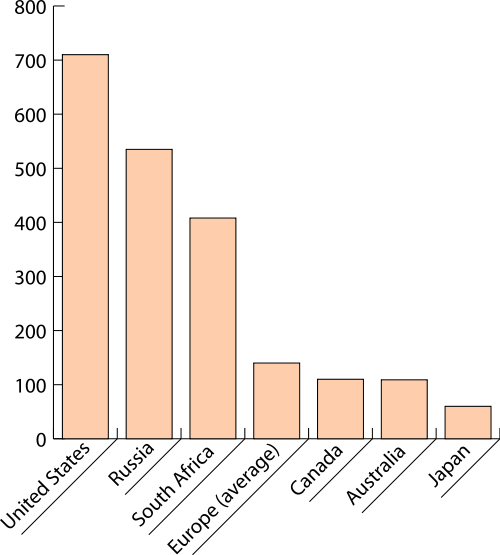
\includegraphics[width=\chartwidth,height=\chartheight]{incarceration}  
\source{Wikipedia}
\end{chart}

\begin{chart}{S}{UL}
\caption{Incarceration ratest across countries}
\label{chart:incarceration}
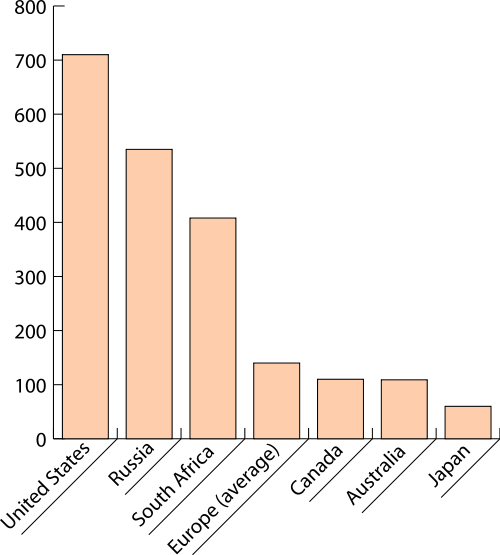
\includegraphics[width=\chartwidth,height=\chartheight]{incarceration}  
\source{Wikipedia}
\end{chart}

\begin{chart}{S}{UR}
\caption{Incarceration ratest across countries}
\label{chart:incarceration}
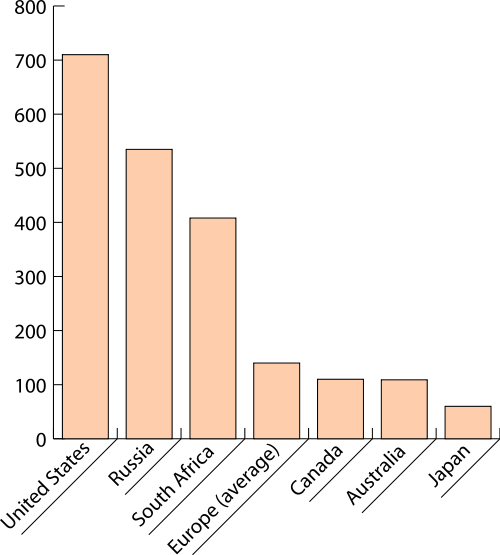
\includegraphics[width=\chartwidth,height=\chartheight]{incarceration}  
\source{Wikipedia}
\end{chart}

\begin{chart}{S}{LR}
\caption{Incarceration ratest across countries}
\label{chart:incarceration}
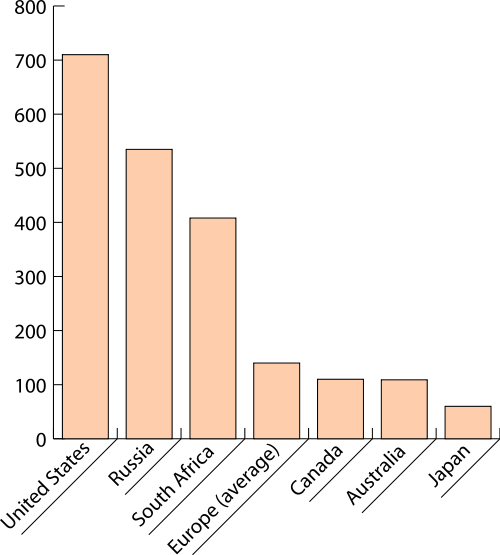
\includegraphics[width=\chartwidth,height=\chartheight]{incarceration}  
\source{Wikipedia}
\end{chart}

\begin{chart}{S}{LL}
\caption{Incarceration ratest across countries}
\label{chart:incarceration}
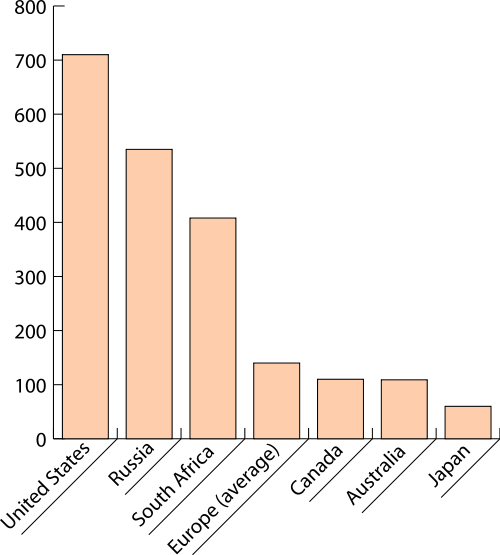
\includegraphics[width=\chartwidth,height=\chartheight]{incarceration}  
\source{Wikipedia}
\end{chart}

%%%%%%%%%%%%%%%%%%%%%%%%%

\section{Environment 1D}

\lipsum[1-4]
%\lipsum[1-5] this breaks it, fills first column

\begin{chart}{S}{ll}
\caption{Incarceration ratest across countries}
\label{chart:incarceration}
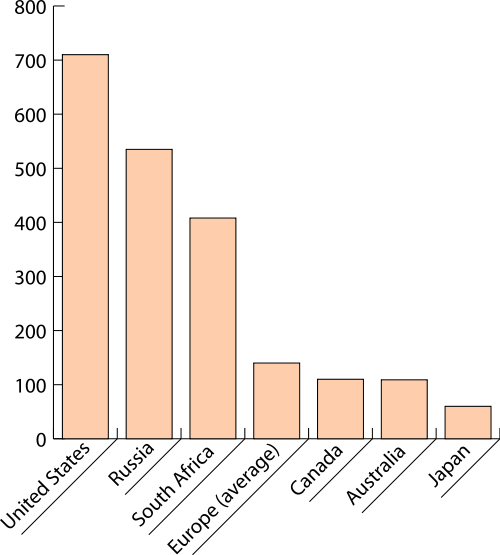
\includegraphics[width=\chartwidth,height=\chartheight]{incarceration}  
\source{Wikipedia}
\end{chart}

\begin{chart}{S}{lr}
\caption{Incarceration ratest across countries}
\label{chart:incarceration}
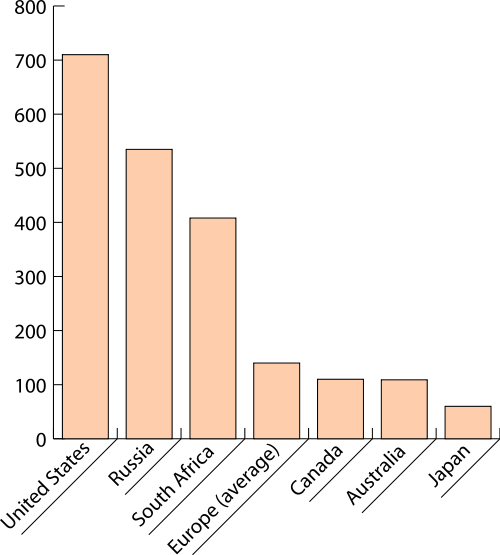
\includegraphics[width=\chartwidth,height=\chartheight]{incarceration}  
\source{Wikipedia}
\end{chart}

\begin{chart}{W}{UL}
\caption{Incarceration ratest across countries}
\label{chart:incarceration}
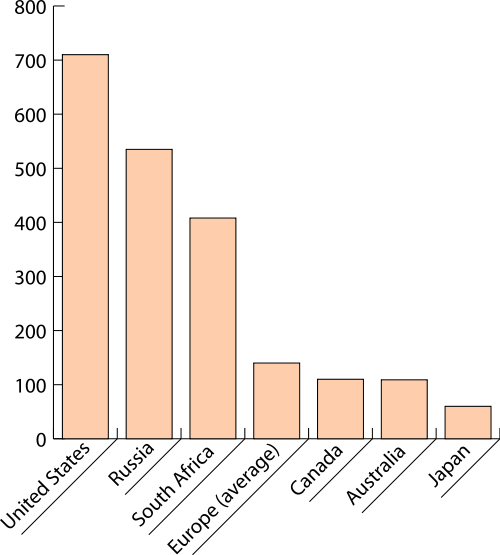
\includegraphics[width=\chartwidth,height=\chartheight]{incarceration}  
\source{Wikipedia}
\end{chart}

\begin{map}{W}{LL}
\caption{Incarceration ratest across countries}
\label{chart:incarceration}
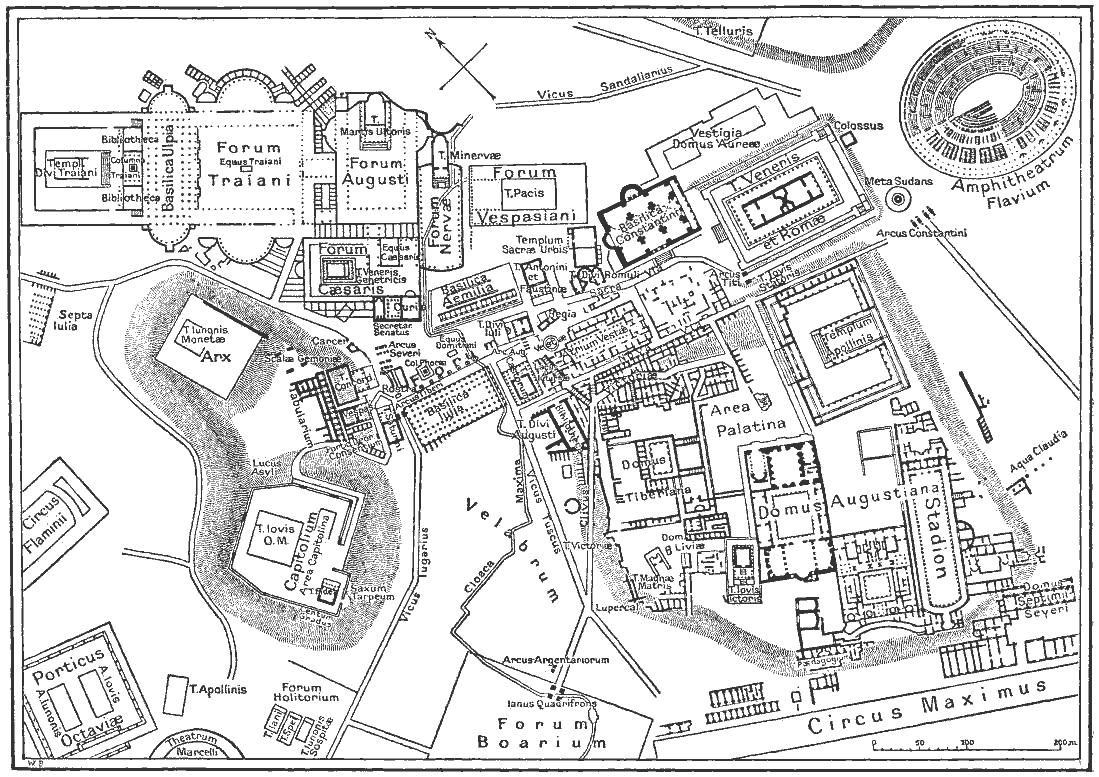
\includegraphics[width=\chartwidth,height=\chartheight]{Rome}  
\source{Wikipedia}
\end{map}

%%%%%%%%%%%%%%%%%%%%%%%%%%%%%%%%

\section{Environment 1E}

\lipsum[1-4]
%\lipsum[1-5] this breaks it, fills first column

\begin{chart}{S}{ll}
\caption{Incarceration ratest across countries}
\label{chart:incarceration}
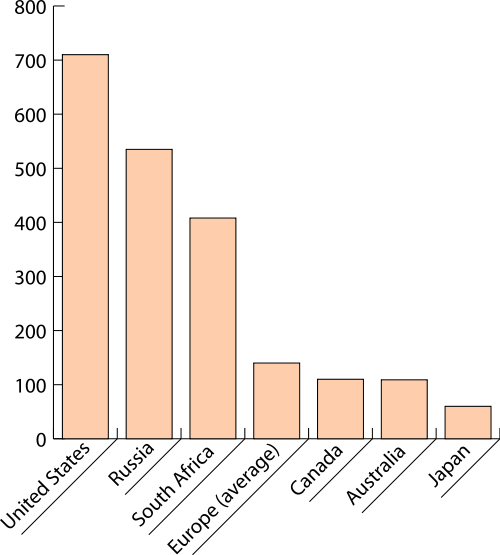
\includegraphics[width=\chartwidth,height=\chartheight]{incarceration}  
\source{Wikipedia}
\end{chart}

\begin{chart}{S}{lr}
\caption{Incarceration ratest across countries}
\label{chart:incarceration}
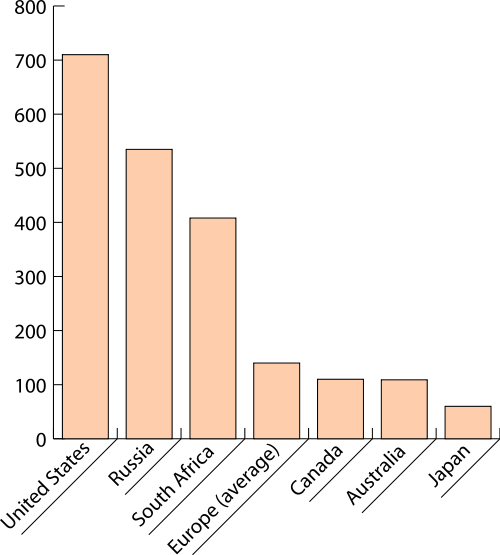
\includegraphics[width=\chartwidth,height=\chartheight]{incarceration}  
\source{Wikipedia}
\end{chart}

\begin{map}{B}{UL}
\caption{Incarceration ratest across countries}
\label{chart:incarceration}
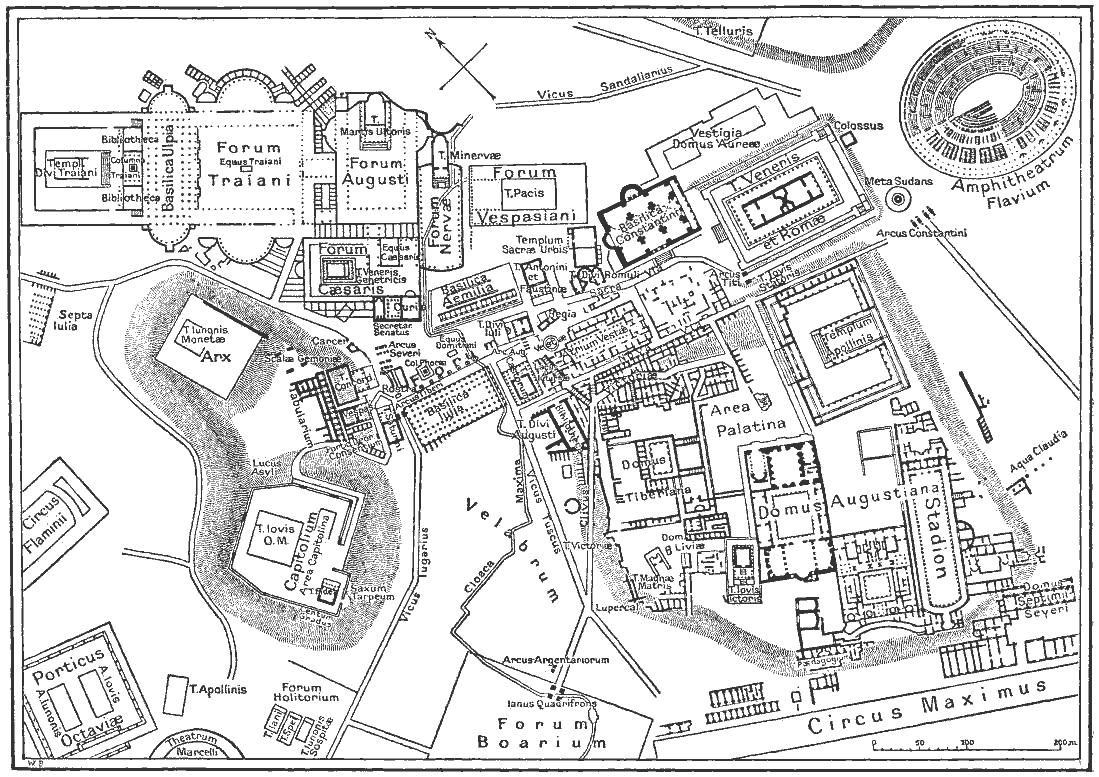
\includegraphics[width=\chartwidth,height=\chartheight]{Rome}  
\source{Wikipedia}
\end{map}

%%%%%%%%%%%%%%%%%%%%%%%%%%%%%%%%%

\section{Environment 2A}

\lipsum[1-2]
%\lipsum[1-5] this breaks it, fills first column

\begin{chart}{S}{ur}
\caption{Incarceration ratest across countries}
\label{chart:incarceration}
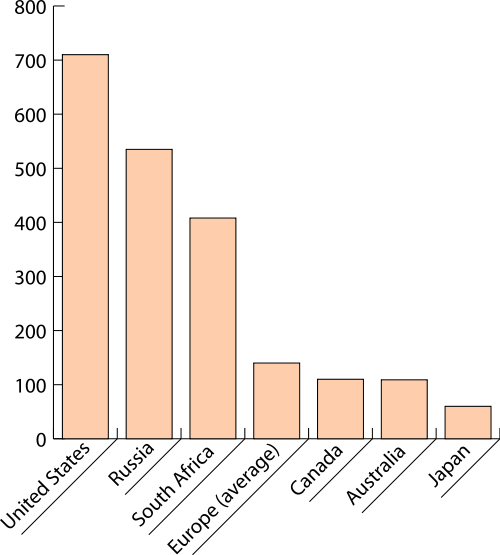
\includegraphics[width=\chartwidth,height=\chartheight]{incarceration}  
\source{Wikipedia}
\end{chart}

\begin{chart}{S}{ll}
\caption{Incarceration ratest across countries}
\label{chart:incarceration}
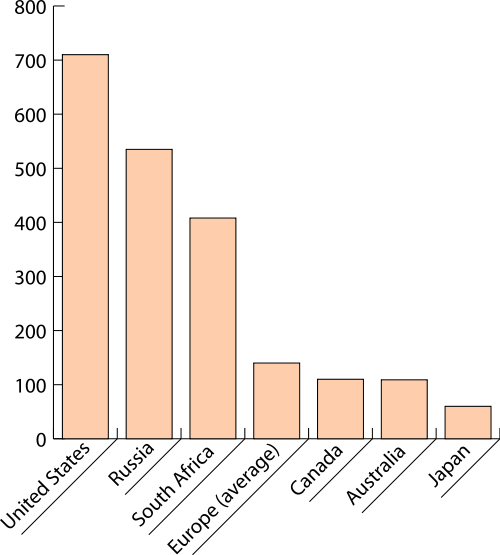
\includegraphics[width=\chartwidth,height=\chartheight]{incarceration}  
\source{Wikipedia}
\end{chart}

\begin{chart}{S}{lr}
\caption{Incarceration ratest across countries}
\label{chart:incarceration}
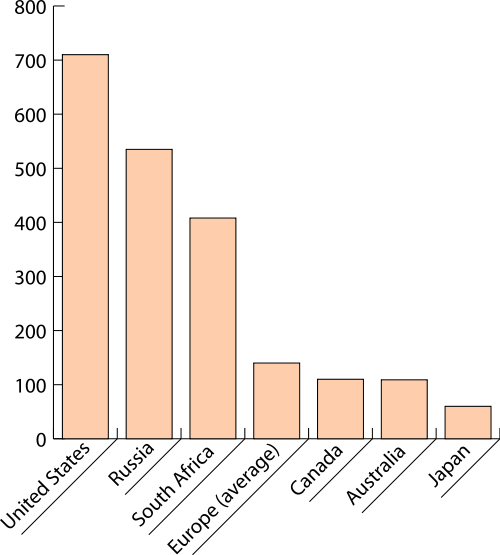
\includegraphics[width=\chartwidth,height=\chartheight]{incarceration}  
\source{Wikipedia}
\end{chart}

\begin{map}{W}{UL}
\caption{Ancient Roma  (Trajan times)}
\label{map:roma}
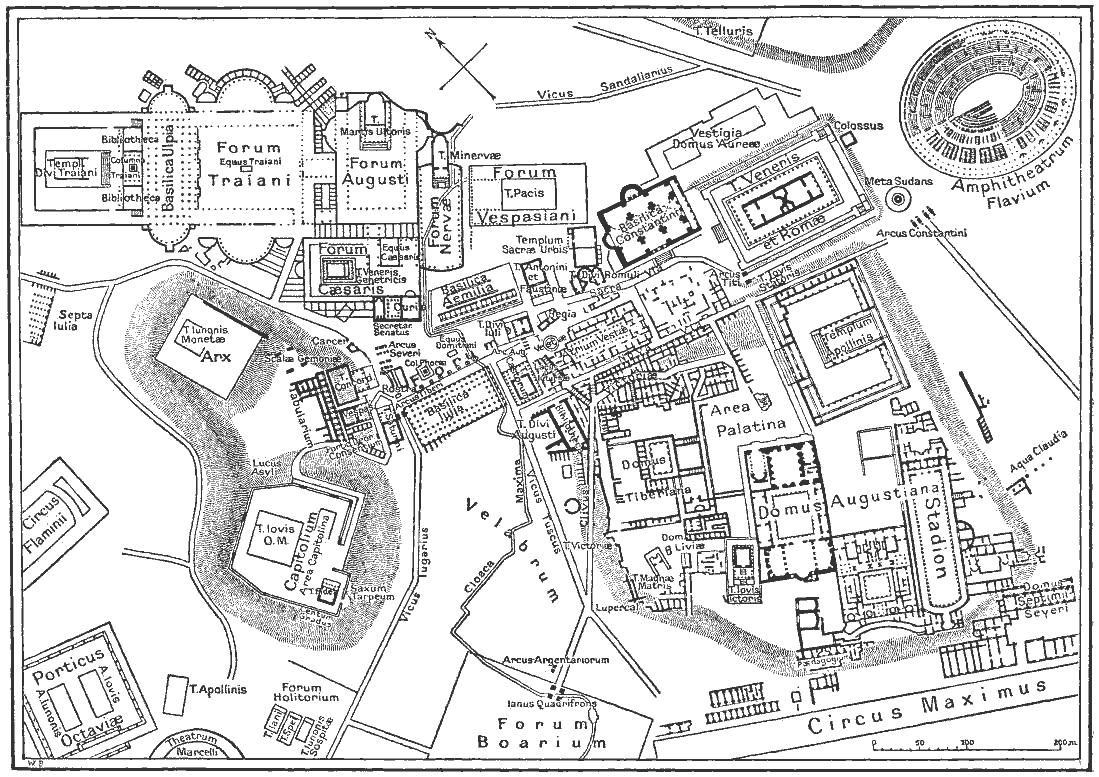
\includegraphics[width=\chartwidth,height=\chartheight]{Rome}
\source{Wikipedia}
\refMetadata{agripop}
\end{map}

\begin{chart}{S}{LL}
\caption{Incarceration ratest across countries}
\label{chart:incarceration}
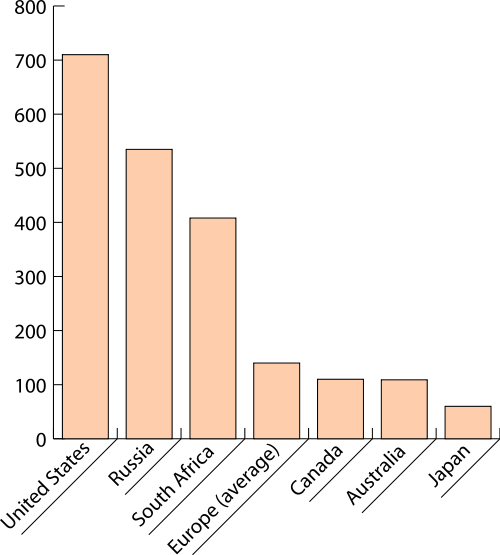
\includegraphics[width=\chartwidth,height=\chartheight]{incarceration}  
\source{Wikipedia}
\end{chart}

\begin{chart}{S}{LR}
\caption{Incarceration ratest across countries}
\label{chart:incarceration}
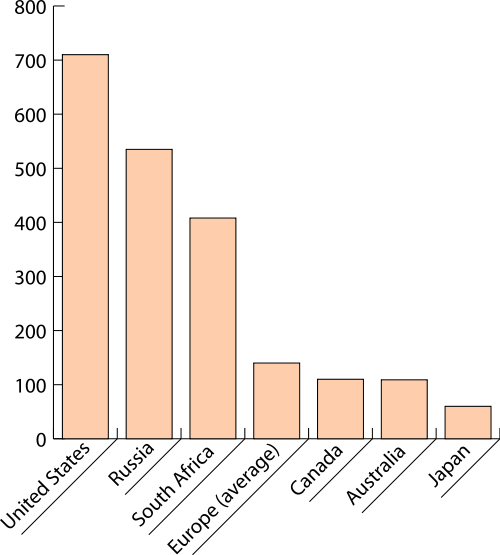
\includegraphics[width=\chartwidth,height=\chartheight]{incarceration}  
\source{Wikipedia}
\end{chart}

%%%%%%%%%%%%%%%%%%%%%%%%%%%%%%%%

%\section{Environment 2B}
%
%\lipsum[1-2]
%
%\begin{chart}{S}{ur}
%\caption{Incarceration ratest across countries}
%\label{chart:incarceration}
%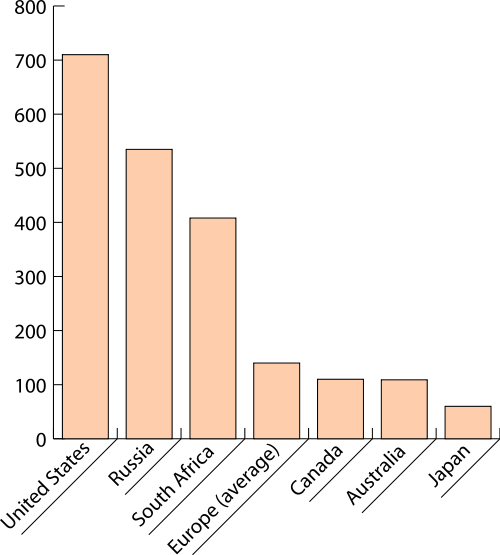
\includegraphics[width=\chartwidth,height=\chartheight]{incarceration}  
%\source{Wikipedia}
%\end{chart}
%
%\begin{chart}{S}{ll}
%\caption{Incarceration ratest across countries}
%\label{chart:incarceration}
%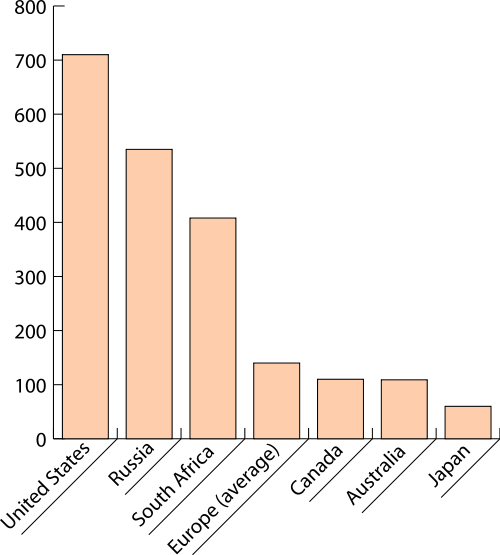
\includegraphics[width=\chartwidth,height=\chartheight]{incarceration}  
%\source{Wikipedia}
%\end{chart}
%
%\begin{chart}{S}{lr}
%\caption{Incarceration ratest across countries}
%\label{chart:incarceration}
%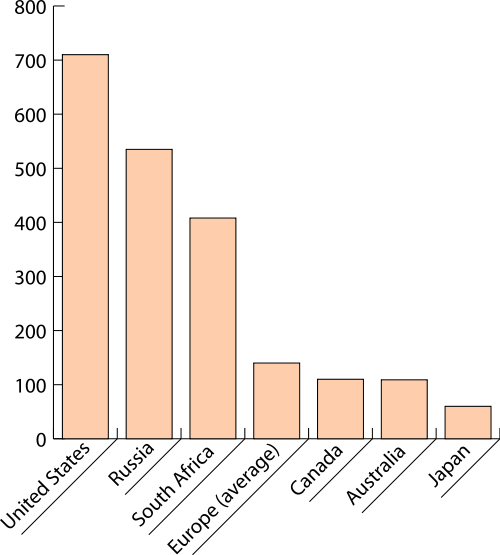
\includegraphics[width=\chartwidth,height=\chartheight]{incarceration}  
%\source{Wikipedia}
%\end{chart}
%
%\begin{chart}{S}{UL}
%\caption{Incarceration ratest across countries}
%\label{chart:incarceration}
%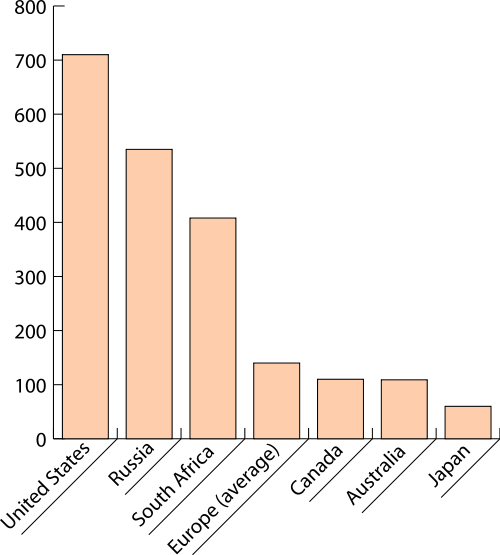
\includegraphics[width=\chartwidth,height=\chartheight]{incarceration}  
%\source{Wikipedia}
%\end{chart}
%
%\begin{chart}{S}{UR}
%\caption{Incarceration ratest across countries}
%\label{chart:incarceration}
%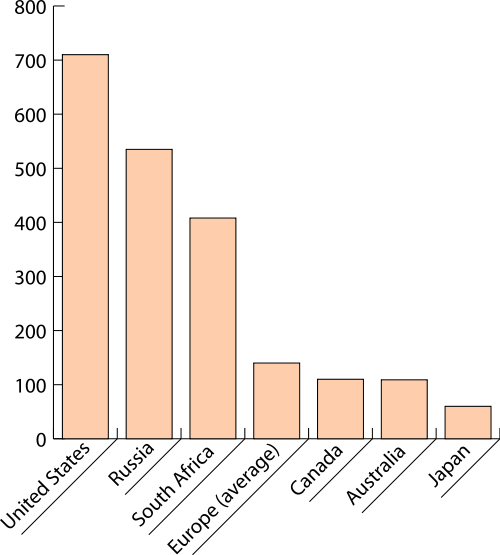
\includegraphics[width=\chartwidth,height=\chartheight]{incarceration}  
%\source{Wikipedia}
%\end{chart}
%
%\begin{map}{W}{LL}
%\caption{Ancient Roma  (Trajan times)}
%\label{map:roma}
%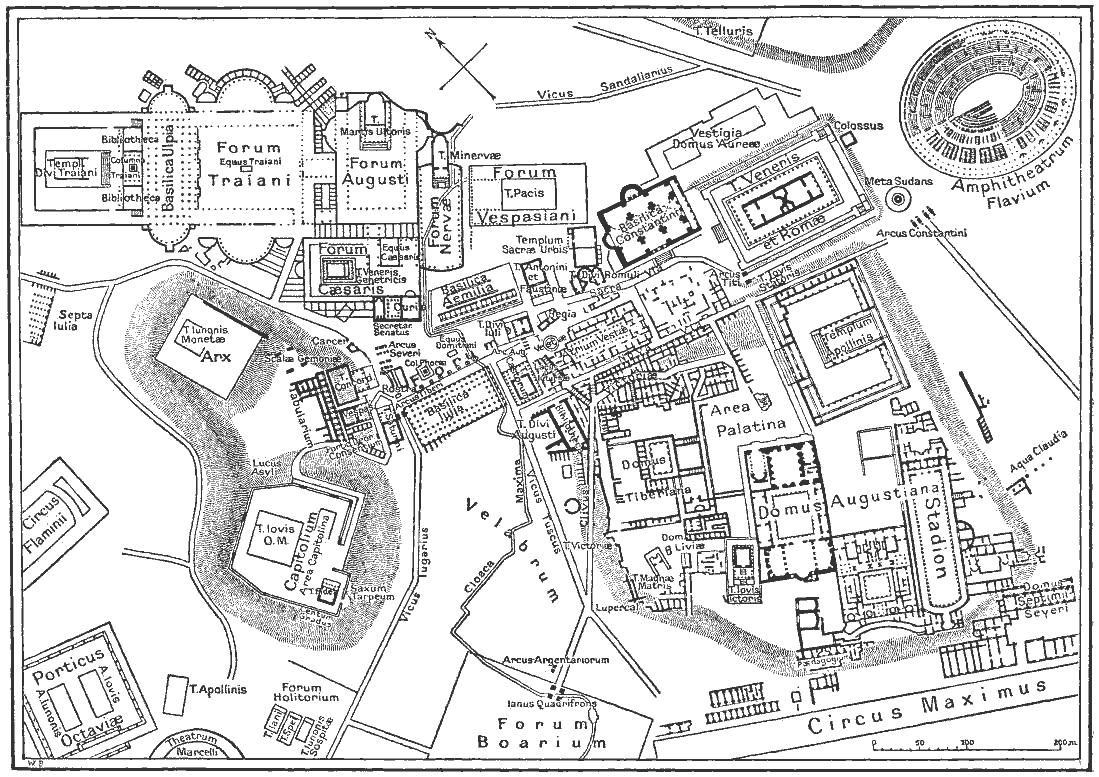
\includegraphics[width=\chartwidth,height=\chartheight]{Rome}
%\source{Wikipedia}
%\refMetadata{agripop}
%\end{map}


%%%%%%%%%%%%%%%%%%%%

\section{Environment 2C}

\lipsum[1-2]
%\lipsum[1-5] this breaks it, fills first column

\begin{chart}{S}{ur}
\caption{Incarceration ratest across countries}
\label{chart:incarceration}
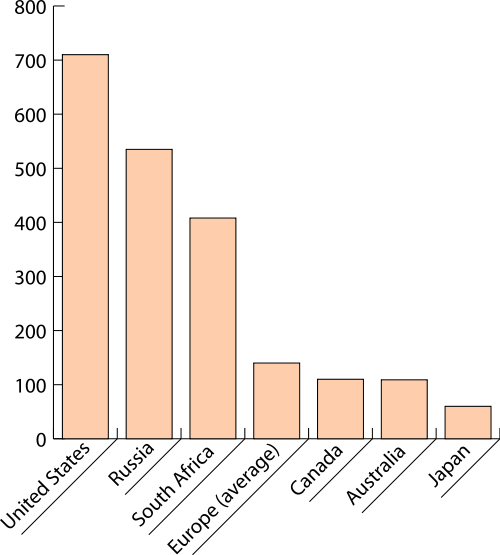
\includegraphics[width=\chartwidth,height=\chartheight]{incarceration}  
\source{Wikipedia}
\end{chart}

\begin{chart}{S}{ll}
\caption{Incarceration ratest across countries}
\label{chart:incarceration}
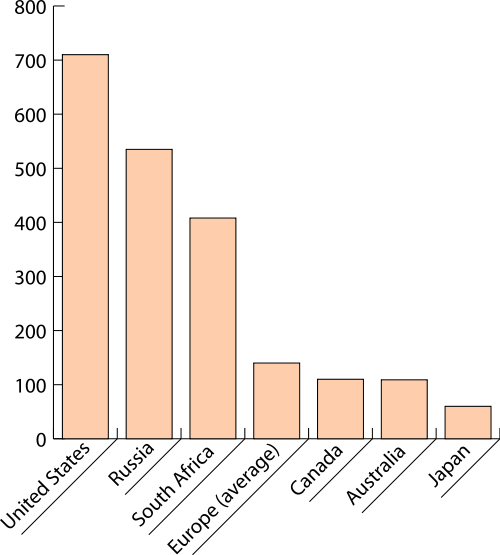
\includegraphics[width=\chartwidth,height=\chartheight]{incarceration}  
\source{Wikipedia}
\end{chart}

\begin{chart}{S}{lr}
\caption{Incarceration ratest across countries}
\label{chart:incarceration}
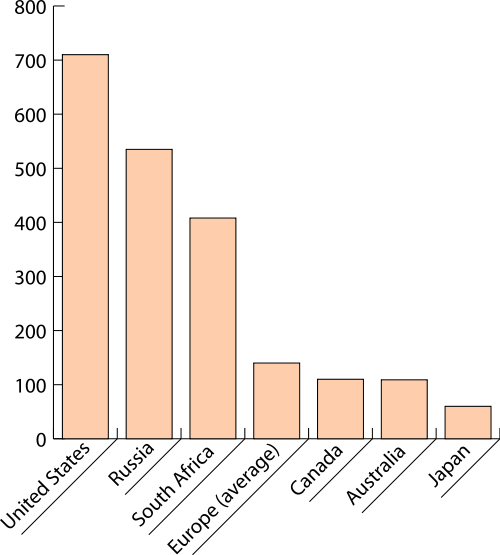
\includegraphics[width=\chartwidth,height=\chartheight]{incarceration}  
\source{Wikipedia}
\end{chart}

\begin{chart}{S}{UL}
\caption{Incarceration ratest across countries}
\label{chart:incarceration}
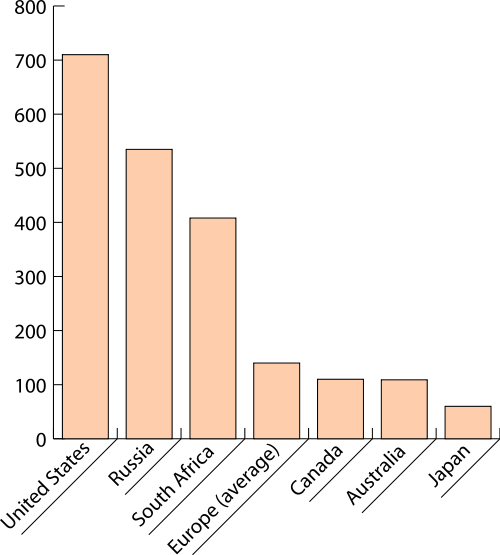
\includegraphics[width=\chartwidth,height=\chartheight]{incarceration}  
\source{Wikipedia}
\end{chart}

\begin{chart}{S}{UR}
\caption{Incarceration ratest across countries}
\label{chart:incarceration}
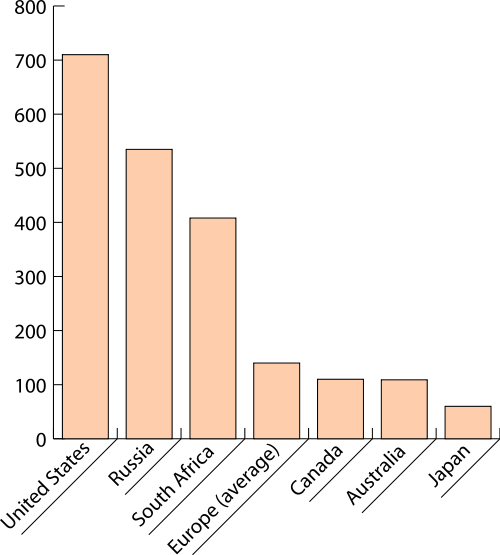
\includegraphics[width=\chartwidth,height=\chartheight]{incarceration}  
\source{Wikipedia}
\end{chart}

\begin{chart}{S}{LR}
\caption{Incarceration ratest across countries}
\label{chart:incarceration}
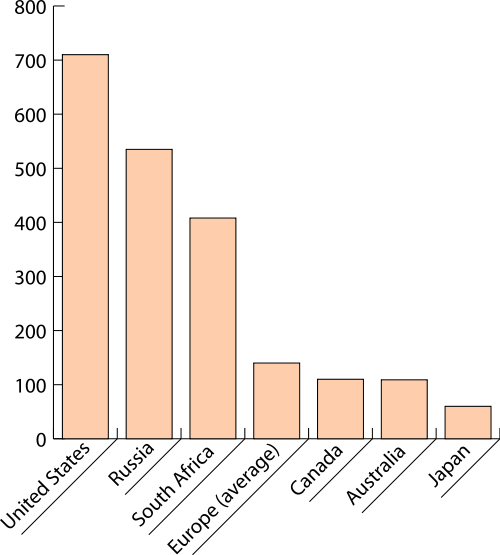
\includegraphics[width=\chartwidth,height=\chartheight]{incarceration}  
\source{Wikipedia}
\end{chart}

\begin{chart}{S}{LL}
\caption{Incarceration ratest across countries}
\label{chart:incarceration}
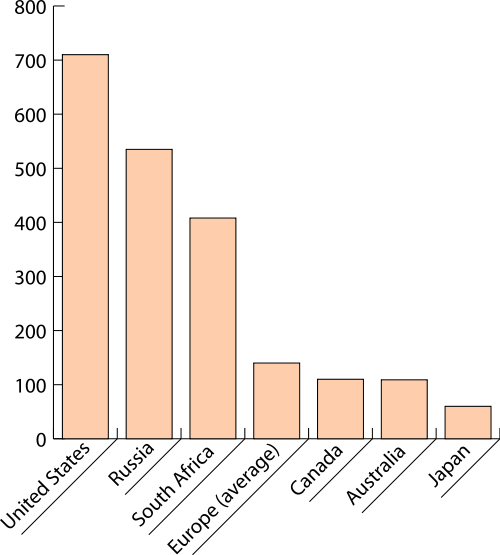
\includegraphics[width=\chartwidth,height=\chartheight]{incarceration}  
\source{Wikipedia}
\end{chart}

%%%%%%%%%%%%%%%%%%%%%%%%%

\section{Environment 2D}

\lipsum[1-2]
%\lipsum[1-5] this breaks it, fills first column

\begin{chart}{S}{ur}
\caption{Incarceration ratest across countries}
\label{chart:incarceration}
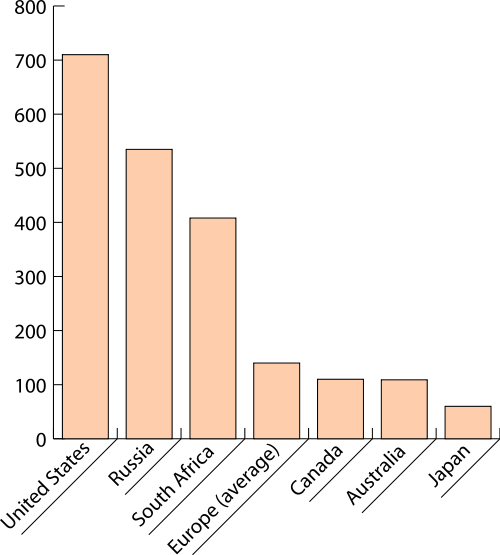
\includegraphics[width=\chartwidth,height=\chartheight]{incarceration}  
\source{Wikipedia}
\end{chart}

\begin{chart}{S}{ll}
\caption{Incarceration ratest across countries}
\label{chart:incarceration}
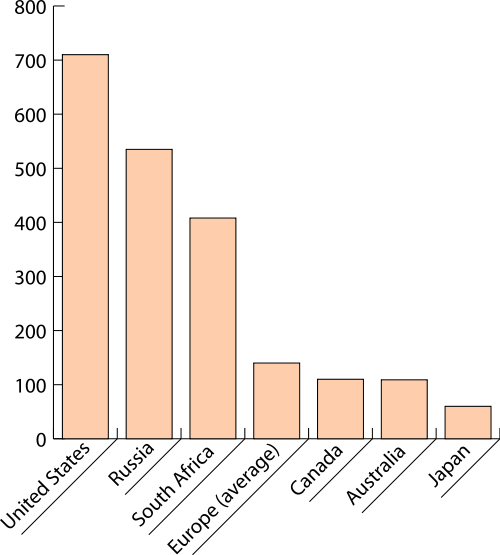
\includegraphics[width=\chartwidth,height=\chartheight]{incarceration}  
\source{Wikipedia}
\end{chart}

\begin{chart}{S}{lr}
\caption{Incarceration ratest across countries}
\label{chart:incarceration}
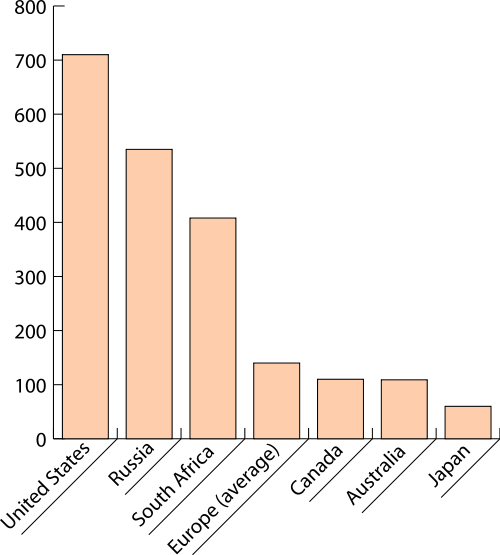
\includegraphics[width=\chartwidth,height=\chartheight]{incarceration}  
\source{Wikipedia}
\end{chart}

\begin{chart}{W}{UL}
\caption{Incarceration ratest across countries}
\label{chart:incarceration}
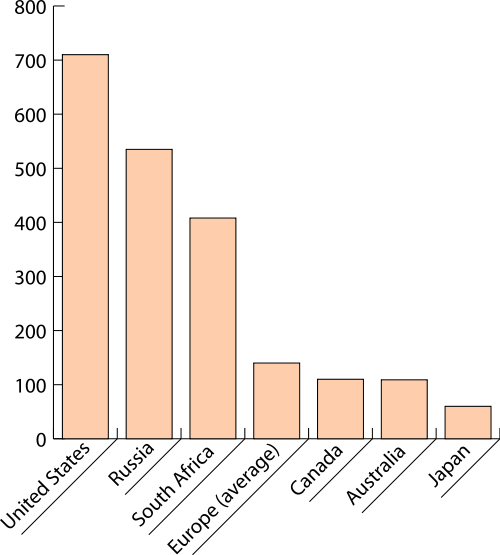
\includegraphics[width=\chartwidth,height=\chartheight]{incarceration}  
\source{Wikipedia}
\end{chart}

\begin{map}{W}{LL}
\caption{Incarceration ratest across countries}
\label{chart:incarceration}
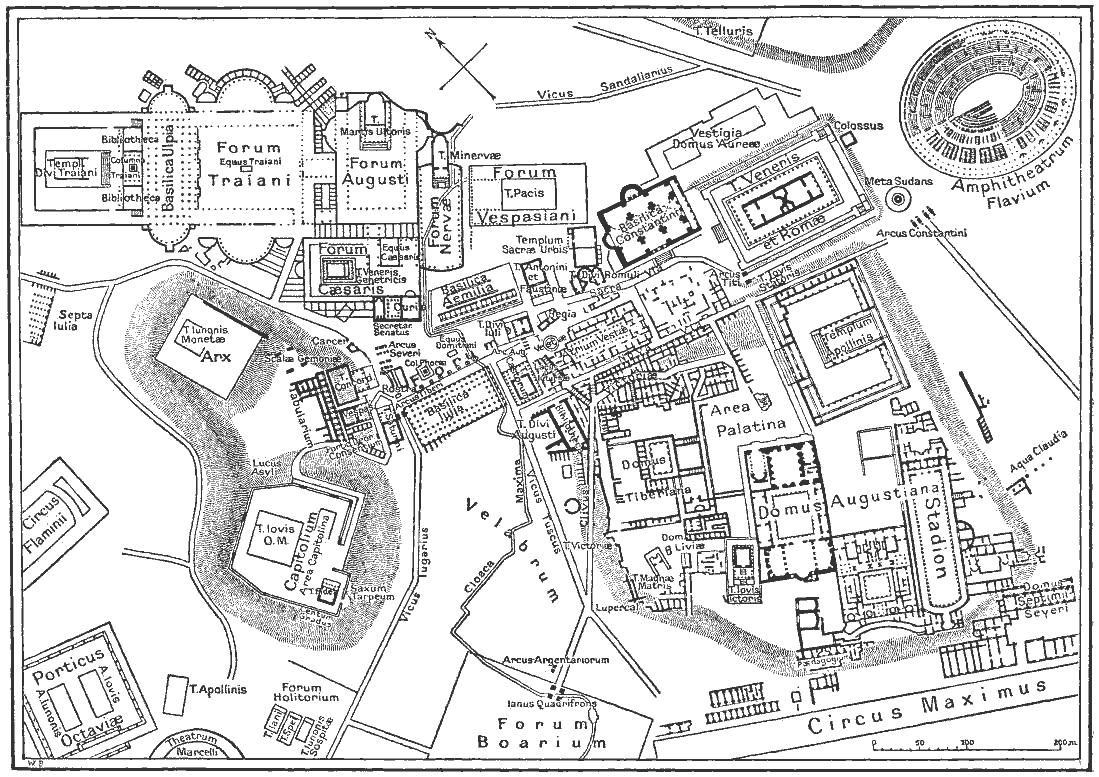
\includegraphics[width=\chartwidth,height=\chartheight]{Rome}  
\source{Wikipedia}
\end{map}

%%%%%%%%%%%%%%%%%%%%%%%%%%%%%%%%

\section{Environment 2E}

\lipsum[1-2]
%\lipsum[1-5] this breaks it, fills first column

\begin{chart}{S}{ur}
\caption{Incarceration ratest across countries}
\label{chart:incarceration}
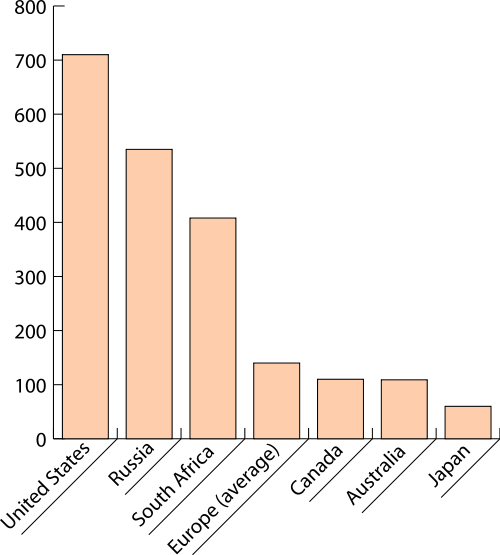
\includegraphics[width=\chartwidth,height=\chartheight]{incarceration}  
\source{Wikipedia}
\end{chart}

\begin{chart}{S}{ll}
\caption{Incarceration ratest across countries}
\label{chart:incarceration}
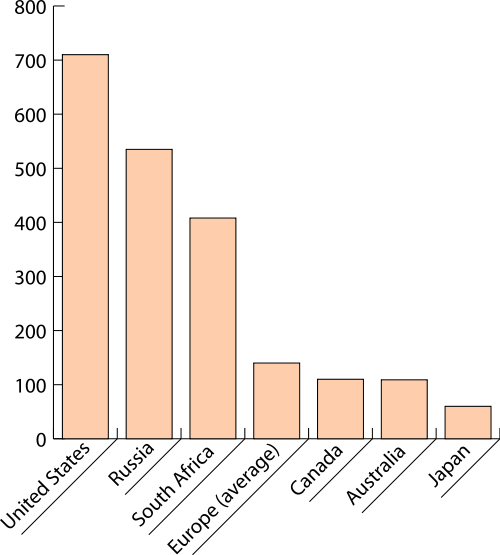
\includegraphics[width=\chartwidth,height=\chartheight]{incarceration}  
\source{Wikipedia}
\end{chart}

\begin{chart}{S}{lr}
\caption{Incarceration ratest across countries}
\label{chart:incarceration}
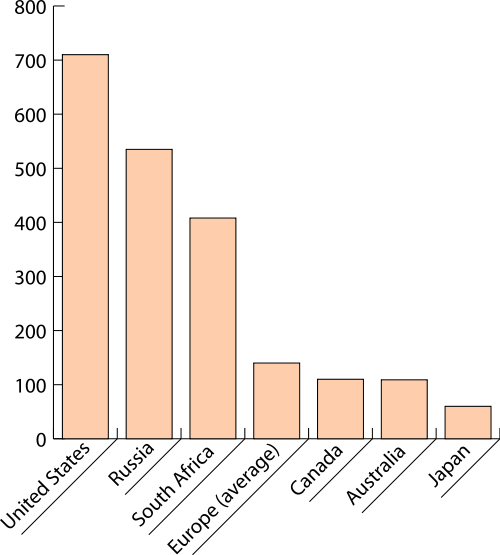
\includegraphics[width=\chartwidth,height=\chartheight]{incarceration}  
\source{Wikipedia}
\end{chart}

\begin{map}{B}{UL}
\caption{Incarceration ratest across countries}
\label{chart:incarceration}
\includegraphics[width=\chartwidth,height=\chartheight]{Rome}  
\source{Wikipedia}
\end{map}

%%%%%%%%%%%%%%%%%%%%%%%%%%%%%%%%%

%\section{Environment 3A}
%
%\lipsum[1-4]
%%\lipsum[1-5] this breaks it, fills first column
%
%\begin{map}{W}{ll}
%\caption{Incarceration ratest across countries}
%\label{chart:incarceration}
%\includegraphics[width=\chartwidth,height=\chartheight]{incarceration}  
%\source{Wikipedia}
%\end{map}
%
%\begin{map}{W}{UL}
%\caption{Ancient Roma  (Trajan times)}
%\label{map:roma}
%\includegraphics[width=\chartwidth,height=\chartheight]{Rome}
%\source{Wikipedia}
%\refMetadata{agripop}
%\end{map}

%\begin{chart}{S}{LL}
%\caption{Incarceration ratest across countries}
%\label{chart:incarceration}
%\includegraphics[width=\chartwidth,height=\chartheight]{incarceration}  
%\source{Wikipedia}
%\end{chart}
%
%\begin{chart}{S}{LR}
%\caption{Incarceration ratest across countries}
%\label{chart:incarceration}
%\includegraphics[width=\chartwidth,height=\chartheight]{incarceration}  
%\source{Wikipedia}
%\end{chart}

%
%
%%\section{Environment 3B}
%
%%\lipsum[1-4]
%%%\lipsum[1-5] this breaks it, fills first column
%%
%%\begin{chart}{W}{ll}
%%\caption{Incarceration ratest across countries}
%%\label{chart:incarceration}
%%\includegraphics[width=\chartwidth,height=\chartheight]{incarceration}  
%%\source{Wikipedia}
%%\end{chart}
%%
%%%\begin{chart}{S}{lr}
%%%\caption{Incarceration ratest across countries}
%%%\label{chart:incarceration}
%%%\includegraphics[width=\chartwidth,height=\chartheight]{incarceration}  
%%%\source{Wikipedia}
%%%\end{chart}
%%
%%\begin{chart}{S}{UL}
%%\caption{Incarceration ratest across countries}
%%\label{chart:incarceration}
%%\includegraphics[width=\chartwidth,height=\chartheight]{incarceration}  
%%\source{Wikipedia}
%%\end{chart}
%%
%%\begin{chart}{S}{UR}
%%\caption{Incarceration ratest across countries}
%%\label{chart:incarceration}
%%\includegraphics[width=\chartwidth,height=\chartheight]{incarceration}  
%%\source{Wikipedia}
%%\end{chart}
%%
%%\begin{map}{W}{LL}
%%\caption{Ancient Roma  (Trajan times)}
%%\label{map:roma}
%%\includegraphics[width=\chartwidth,height=\chartheight]{Rome}
%%\source{Wikipedia}
%%\refMetadata{agripop}
%%\end{map}
%
%
%%%%%%%%%%%%%%%%%%%%%
%
%%\section{Environment 3C}
%%
%%\lipsum[1-4]
%%%\lipsum[1-5] this breaks it, fills first column
%%
%%\begin{chart}{W}{ll}
%%\caption{Incarceration ratest across countries}
%%\label{chart:incarceration}
%%\includegraphics[width=\chartwidth,height=\chartheight]{incarceration}  
%%\source{Wikipedia}
%%\end{chart}
%%
%%%\begin{chart}{S}{lr}
%%%\caption{Incarceration ratest across countries}
%%%\label{chart:incarceration}
%%%\includegraphics[width=\chartwidth,height=\chartheight]{incarceration}  
%%%\source{Wikipedia}
%%%\end{chart}
%%
%%\begin{chart}{S}{UL}
%%\caption{Incarceration ratest across countries}
%%\label{chart:incarceration}
%%\includegraphics[width=\chartwidth,height=\chartheight]{incarceration}  
%%\source{Wikipedia}
%%\end{chart}
%%
%%\begin{chart}{S}{UR}
%%\caption{Incarceration ratest across countries}
%%\label{chart:incarceration}
%%\includegraphics[width=\chartwidth,height=\chartheight]{incarceration}  
%%\source{Wikipedia}
%%\end{chart}
%%
%%\begin{chart}{S}{LR}
%%\caption{Incarceration ratest across countries}
%%\label{chart:incarceration}
%%\includegraphics[width=\chartwidth,height=\chartheight]{incarceration}  
%%\source{Wikipedia}
%%\end{chart}
%%
%%\begin{chart}{S}{LL}
%%\caption{Incarceration ratest across countries}
%%\label{chart:incarceration}
%%\includegraphics[width=\chartwidth,height=\chartheight]{incarceration}  
%%\source{Wikipedia}
%%\end{chart}
%%
%%%%%%%%%%%%%%%%%%%%%%%%%%%
%%
%%\section{Environment 3D}
%%
%%\lipsum[1-4]
%%%\lipsum[1-5] this breaks it, fills first column
%%
%%\begin{map}{W}{ll}
%%\caption{Incarceration ratest across countries}
%%\label{chart:incarceration}
%%\includegraphics[width=\chartwidth,height=\chartheight]{incarceration}  
%%\source{Wikipedia}
%%\end{map}
%%%
%%%\begin{chart}{S}{lr}
%%%\caption{Incarceration ratest across countries}
%%%\label{chart:incarceration}
%%%\includegraphics[width=\chartwidth,height=\chartheight]{incarceration}  
%%%\source{Wikipedia}
%%%\end{chart}
%%
%%\begin{chart}{W}{UL}
%%\caption{Incarceration ratest across countries}
%%\label{chart:incarceration}
%%\includegraphics[width=\chartwidth,height=\chartheight]{incarceration}  
%%\source{Wikipedia}
%%\end{chart}
%%
%%\begin{map}{W}{LL}
%%\caption{Incarceration ratest across countries}
%%\label{chart:incarceration}
%%\includegraphics[width=\chartwidth,height=\chartheight]{Rome}  
%%\source{Wikipedia}
%%\end{map}
%%
%%%%%%%%%%%%%%%%%%%%%%%%%%%%%%%%%%
%%
%%\section{Environment 3E}
%%
%%\lipsum[1-4]
%%%\lipsum[1-5] this breaks it, fills first column
%%
%%\begin{chart}{W}{ll}
%%\caption{Incarceration ratest across countries}
%%\label{chart:incarceration}
%%\includegraphics[width=\chartwidth,height=\chartheight]{incarceration}  
%%\source{Wikipedia}
%%\end{chart}
%%
%%%\begin{chart}{S}{lr}
%%%\caption{Incarceration ratest across countries}
%%%\label{chart:incarceration}
%%%\includegraphics[width=\chartwidth,height=\chartheight]{incarceration}  
%%%\source{Wikipedia}
%%%\end{chart}
%%
%%\begin{map}{B}{UL}
%%\caption{Incarceration ratest across countries}
%%\label{chart:incarceration}
%%\includegraphics[width=\chartwidth,height=\chartheight]{Rome}  
%%\source{Wikipedia}
%%\end{map}
%
%%%%%%%%%%%%%%%%%%%%%%%%%%%%%%%%%%
%
%
%%%%%%%%%%%%%%%%%%%%%%%%%%%%%%%%%%

%\section{Environment 4A}
%
%\lipsum[1-2]
%%\lipsum[1-5] this breaks it, fills first column
%
%\begin{map}{S}{ur}
%\caption{Incarceration ratest across countries}
%\label{chart:incarceration}
%\includegraphics[width=\chartwidth,height=\chartheight]{incarceration}  
%\source{Wikipedia}
%\end{map}
%
%\begin{map}{W}{ll}
%\caption{Incarceration ratest across countries}
%\label{chart:incarceration}
%\includegraphics[width=\chartwidth,height=\chartheight]{incarceration}  
%\source{Wikipedia}
%\end{map}
%
%\begin{map}{W}{UL}
%\caption{Ancient Roma  (Trajan times)}
%\label{map:roma}
%\includegraphics[width=\chartwidth,height=\chartheight]{Rome}
%\source{Wikipedia}
%\refMetadata{agripop}
%\end{map}
%
%\begin{chart}{S}{LL}
%\caption{Incarceration ratest across countries}
%\label{chart:incarceration}
%\includegraphics[width=\chartwidth,height=\chartheight]{incarceration}  
%\source{Wikipedia}
%\end{chart}
%
%\begin{chart}{S}{LR}
%\caption{Incarceration ratest across countries}
%\label{chart:incarceration}
%\includegraphics[width=\chartwidth,height=\chartheight]{incarceration}  
%\source{Wikipedia}
%\end{chart}

%%%%%%%%%%%%%%%%%%%%%%%%%%%

\section{Environment 5A}

\lipsum[1-2]
%\lipsum[1-5] this breaks it, fills first column

\begin{map}{T}{ur}
\caption{Incarceration ratest across countries}
\label{chart:incarceration}
\includegraphics[width=\chartwidth,height=\chartheight]{incarceration}  
\source{Wikipedia}
\end{map}

\begin{map}{S}{ll}
\caption{Incarceration ratest across countries}
\label{chart:incarceration}
\includegraphics[width=\chartwidth,height=\chartheight]{incarceration}  
\source{Wikipedia}
\end{map}

\begin{map}{W}{UL}
\caption{Ancient Roma  (Trajan times)}
\label{map:roma}
\includegraphics[width=\chartwidth,height=\chartheight]{Rome}
\source{Wikipedia}
\refMetadata{agripop}
\end{map}

\begin{chart}{S}{LL}
\caption{Incarceration ratest across countries}
\label{chart:incarceration}
\includegraphics[width=\chartwidth,height=\chartheight]{incarceration}  
\source{Wikipedia}
\end{chart}

\begin{chart}{S}{LR}
\caption{Incarceration ratest across countries}
\label{chart:incarceration}
\includegraphics[width=\chartwidth,height=\chartheight]{incarceration}  
\source{Wikipedia}
\end{chart}

%%%%%%%%%%%%%%%%%%%%%%%%%%%

%\section{Environment 5B}
%
%\lipsum[1-2]
%%\lipsum[1-5] this breaks it, fills first column
%
%\begin{map}{T}{ur}
%\caption{Incarceration ratest across countries}
%\label{chart:incarceration}
%\includegraphics[width=\chartwidth,height=\chartheight]{incarceration}  
%\source{Wikipedia}
%\end{map}
%
%\begin{map}{S}{ll}
%\caption{Incarceration ratest across countries}
%\label{chart:incarceration}
%\includegraphics[width=\chartwidth,height=\chartheight]{Rome}  
%\source{Wikipedia}
%\end{map}
%
%\begin{chart}{S}{UL}
%\caption{Incarceration ratest across countries}
%\label{chart:incarceration}
%\includegraphics[width=\chartwidth,height=\chartheight]{incarceration}  
%\source{Wikipedia}
%\end{chart}
%
%\begin{chart}{S}{UR}
%\caption{Incarceration ratest across countries}
%\label{chart:incarceration}
%\includegraphics[width=\chartwidth,height=\chartheight]{incarceration}  
%\source{Wikipedia}
%\end{chart}
%
%\begin{map}{W}{LL}
%\caption{Ancient Roma  (Trajan times)}
%\label{map:roma}
%\includegraphics[width=\chartwidth,height=\chartheight]{Rome}
%\source{Wikipedia}
%\refMetadata{agripop}
%\end{map}

%%%%%%%%%%%%%%%%%%%%%%%%%%%%%%%%%%%

\section{Environment 5C}

\lipsum[1-2]
%\lipsum[1-5] this breaks it, fills first column

\begin{map}{T}{ur}
\caption{Incarceration ratest across countries}
\label{chart:incarceration}
\includegraphics[width=\chartwidth,height=\chartheight]{incarceration}  
\source{Wikipedia}
\end{map}

\begin{map}{S}{ll}
\caption{Incarceration ratest across countries}
\label{chart:incarceration}
\includegraphics[width=\chartwidth,height=\chartheight]{Rome}  
\source{Wikipedia}
\end{map}

\begin{chart}{S}{UL}
\caption{Incarceration ratest across countries}
\label{chart:incarceration}
\includegraphics[width=\chartwidth,height=\chartheight]{incarceration}  
\source{Wikipedia}
\end{chart}

\begin{chart}{S}{UR}
\caption{Incarceration ratest across countries}
\label{chart:incarceration}
\includegraphics[width=\chartwidth,height=\chartheight]{Rome}  
\source{Wikipedia}
\end{chart}

\begin{chart}{S}{LL}
\caption{Incarceration ratest across countries}
\label{chart:incarceration}
\includegraphics[width=\chartwidth,height=\chartheight]{incarceration}  
\source{Wikipedia}
\end{chart}

\begin{chart}{S}{LR}
\caption{Incarceration ratest across countries}
\label{chart:incarceration}
\includegraphics[width=\chartwidth,height=\chartheight]{incarceration}  
\source{Wikipedia}
\end{chart}

%%%%%%%%%%%%%%%%%%%%%%%%%%%%%%%%%%%%

\section{Environment 5D}

\lipsum[1-2]
%\lipsum[1-5] this breaks it, fills first column

\begin{map}{T}{ur}
\caption{Incarceration ratest across countries}
\label{chart:incarceration}
\includegraphics[width=\chartwidth,height=\chartheight]{incarceration}  
\source{Wikipedia}
\end{map}

\begin{map}{S}{ll}
\caption{Incarceration ratest across countries}
\label{chart:incarceration}
\includegraphics[width=\chartwidth,height=\chartheight]{Rome}  
\source{Wikipedia}
\end{map}

\begin{chart}{W}{UL}
\caption{Incarceration ratest across countries}
\label{chart:incarceration}
\includegraphics[width=\chartwidth,height=\chartheight]{incarceration}  
\source{Wikipedia}
\end{chart}

\begin{map}{W}{LL}
\caption{Incarceration ratest across countries}
\label{chart:incarceration}
\includegraphics[width=\chartwidth,height=\chartheight]{Rome}  
\source{Wikipedia}
\end{map}
%
%%%%%%%%%%%%%%%%%%%%%%%%%%%%%%%%%%%%%
%
\section{Environment 5E}

\lipsum[1-2]
%\lipsum[1-5] this breaks it, fills first column

\begin{map}{T}{ur}
\caption{Incarceration ratest across countries}
\label{chart:incarceration}
\includegraphics[width=\chartwidth,height=\chartheight]{incarceration}  
\source{Wikipedia}
\end{map}

\begin{map}{S}{ll}
\caption{Incarceration ratest across countries}
\label{chart:incarceration}
\includegraphics[width=\chartwidth,height=\chartheight]{Rome}  
\source{Wikipedia}
\end{map}

\begin{chart}{B}{UL}
\caption{Incarceration ratest across countries}
\label{chart:incarceration}
\includegraphics[width=\chartwidth,height=\chartheight]{incarceration}  
\source{Wikipedia}
\end{chart}


%%%%%%%%%%%%%%%%%%%%%%%%%%%%%%%%%%%%

\section{Environment 6A}

\lipsum[1-4]

\begin{map}{T}{ur}
\caption{Incarceration ratest across countries}
\label{chart:incarceration}
\includegraphics[width=\chartwidth,height=\chartheight]{incarceration}  
\source{Wikipedia}
\end{map}

\begin{map}{W}{UL}
\caption{Ancient Roma  (Trajan times)}
\label{map:roma}
\includegraphics[width=\chartwidth,height=\chartheight]{Rome}
\source{Wikipedia}
\refMetadata{agripop}
\end{map}

\begin{chart}{S}{LL}
\caption{Incarceration ratest across countries}
\label{chart:incarceration}
\includegraphics[width=\chartwidth,height=\chartheight]{incarceration}  
\source{Wikipedia}
\end{chart}

\begin{chart}{S}{LR}
\caption{Incarceration ratest across countries}
\label{chart:incarceration}
\includegraphics[width=\chartwidth,height=\chartheight]{incarceration}  
\source{Wikipedia}
\end{chart}

%%%%%%%%%%%%%%%%%%%%%%%%%%%

%\section{Environment 6B}
%
%\lipsum[1-2]
%%\lipsum[1-5] this breaks it, fills first column
%
%\begin{map}{T}{ur}
%\caption{Incarceration ratest across countries}
%\label{chart:incarceration}
%\includegraphics[width=\chartwidth,height=\chartheight]{incarceration}  
%\source{Wikipedia}
%\end{map}
%
%\begin{map}{S}{ll}
%\caption{Incarceration ratest across countries}
%\label{chart:incarceration}
%\includegraphics[width=\chartwidth,height=\chartheight]{Rome}  
%\source{Wikipedia}
%\end{map}
%
%\begin{chart}{S}{UL}
%\caption{Incarceration ratest across countries}
%\label{chart:incarceration}
%\includegraphics[width=\chartwidth,height=\chartheight]{incarceration}  
%\source{Wikipedia}
%\end{chart}
%
%\begin{chart}{S}{UR}
%\caption{Incarceration ratest across countries}
%\label{chart:incarceration}
%\includegraphics[width=\chartwidth,height=\chartheight]{incarceration}  
%\source{Wikipedia}
%\end{chart}
%
%\begin{map}{W}{LL}
%\caption{Ancient Roma  (Trajan times)}
%\label{map:roma}
%\includegraphics[width=\chartwidth,height=\chartheight]{Rome}
%\source{Wikipedia}
%\refMetadata{agripop}
%\end{map}

%%%%%%%%%%%%%%%%%%%%%%%%%%%%%%%%%%%

\section{Environment 6C}

\lipsum[1-4]

\begin{map}{T}{ur}
\caption{Incarceration ratest across countries}
\label{chart:incarceration}
\includegraphics[width=\chartwidth,height=\chartheight]{incarceration}  
\source{Wikipedia}
\end{map}

\begin{chart}{S}{UL}
\caption{Incarceration ratest across countries}
\label{chart:incarceration}
\includegraphics[width=\chartwidth,height=\chartheight]{incarceration}  
\source{Wikipedia}
\end{chart}

\begin{chart}{S}{UR}
\caption{Incarceration ratest across countries}
\label{chart:incarceration}
\includegraphics[width=\chartwidth,height=\chartheight]{Rome}  
\source{Wikipedia}
\end{chart}

\begin{chart}{S}{LL}
\caption{Incarceration ratest across countries}
\label{chart:incarceration}
\includegraphics[width=\chartwidth,height=\chartheight]{incarceration}  
\source{Wikipedia}
\end{chart}

\begin{chart}{S}{LR}
\caption{Incarceration ratest across countries}
\label{chart:incarceration}
\includegraphics[width=\chartwidth,height=\chartheight]{incarceration}  
\source{Wikipedia}
\end{chart}

%%%%%%%%%%%%%%%%%%%%%%%%%%%%%%%%%%%%

\section{Environment 6D}

\lipsum[1-4]

\begin{chart}{T}{ur}
\caption{Incarceration ratest across countries}
\label{chart:incarceration}
\includegraphics[width=\chartwidth,height=\chartheight]{incarceration}  
\source{Wikipedia}
\end{chart}

\begin{chart}{W}{UL}
\caption{Incarceration ratest across countries}
\label{chart:incarceration}
\includegraphics[width=\chartwidth,height=\chartheight]{incarceration}  
\source{Wikipedia}
\end{chart}

\begin{map}{W}{LL}
\caption{Incarceration ratest across countries}
\label{chart:incarceration}
\includegraphics[width=\chartwidth,height=\chartheight]{Rome}  
\source{Wikipedia}
\end{map}
%
%%%%%%%%%%%%%%%%%%%%%%%%%%%%%%%%%%%%%
%
\section{Environment 6E}

\lipsum[1-4]

\begin{chart}{T}{ur}
\caption{Incarceration ratest across countries}
\label{chart:incarceration}
\includegraphics[width=\chartwidth,height=\chartheight]{incarceration}  
\source{Wikipedia}
\end{chart}

\begin{chart}{B}{UL}
\caption{Incarceration ratest across countries}
\label{chart:incarceration}
\includegraphics[width=\chartwidth,height=\chartheight]{incarceration}  
\source{Wikipedia}
\end{chart}

%%%%%%%%%%%%%%%%%%%%%%%%%%%%%%%%%%%%%
%
\section{Environment 7A}

\lipsum[1-4]

\begin{chart}{T}{ur}
\caption{Incarceration ratest across countries}
\label{chart:incarceration}
\includegraphics[width=\chartwidth,height=\chartheight]{incarceration}  
\source{Wikipedia}
\end{chart}

\begin{map}{B}{UL}
\caption{Incarceration ratest across countries}
\label{chart:incarceration}
\includegraphics[width=\chartwidth,height=\chartheight]{Rome}  
\source{Wikipedia}
\end{map}

